\section{Hardware}
Při vytváření stanice bylo nejprve potřeba zvolit vhodný micropočítač pro připojení měřicích komponentů. Nakonec jsme vybrali platformu Arduino,
konkrétně model ESP8266WiFi, který nám umožnil, nejen zapojit všechny různé komponenty potřebné pro měření, ale i připojení k internetu.

Stanice při spuštění zavolá funkci setup, která zinicializuje proměnné potřebné pro běh programu. 
Dále stanice měří počasí a po každých pěti minutách stanice pošle data na server, kde budou dále spracovány.

\begin{figure}[!htb]
   \begin{minipage}{0.48\textwidth}
     \centering
     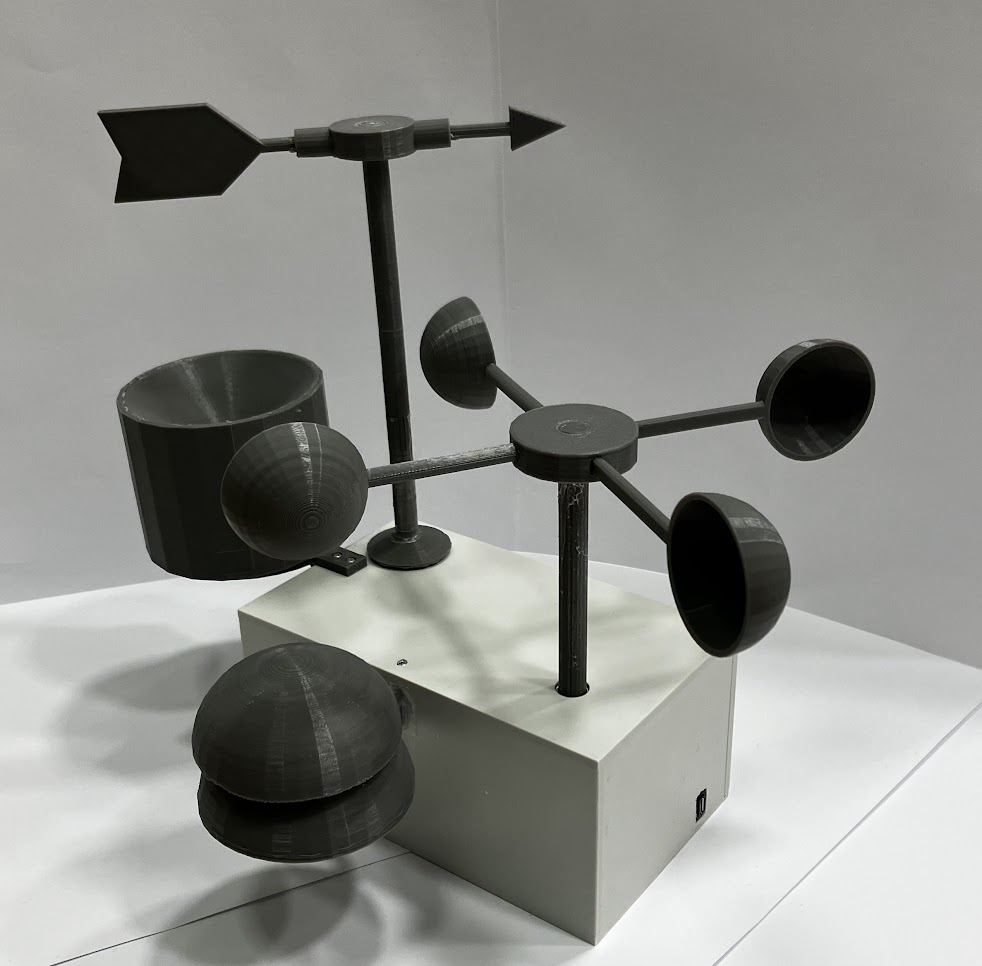
\includegraphics[width=.7\linewidth]{images/stanice0.jpg}
     \caption{Stanice}
   \end{minipage}\hfill
   \begin{minipage}{0.5\textwidth}
     \centering
     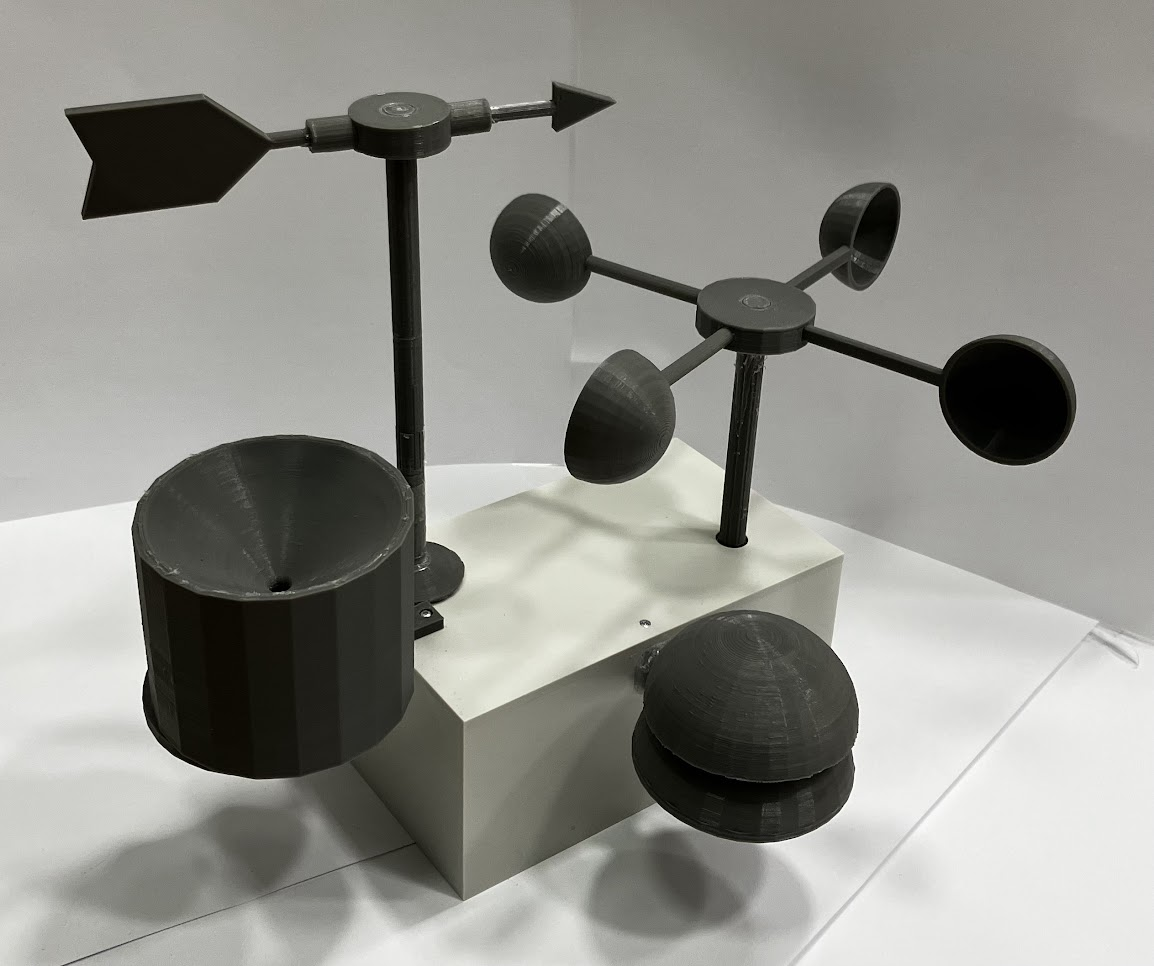
\includegraphics[width=.7\linewidth]{images/stanice1.jpg}
     \caption{Stanice}
   \end{minipage}
\end{figure}
\subsection{Propojení se serverem}
Po zapnutí se stanice připojí k internetu za pomoci WiFi a zaregistruje na backendu (popsáno v kapitole \ref{komunikace}). Jakmile stanice dostane od serveru odpověď s 
JSON Web Tokenem, uloží si ho a při každém odeslání dat na server ho použije k prokázání totožnosti.

\subsection{Měření teploty a vlhkosti}
Pro měření teploty a vlhkosti byl použit Digitální teploměr Adafruit AM2320 Senzor\cite{teplomer}. V tomto případě nebylo zapotřebí vymýšlet jak cokoliv měřit,
protože senzor je připojen přes I2C interface, ze kterého program přímo čte již naměřené hodnoty.
\begin{figure}[h] 
    \centering
    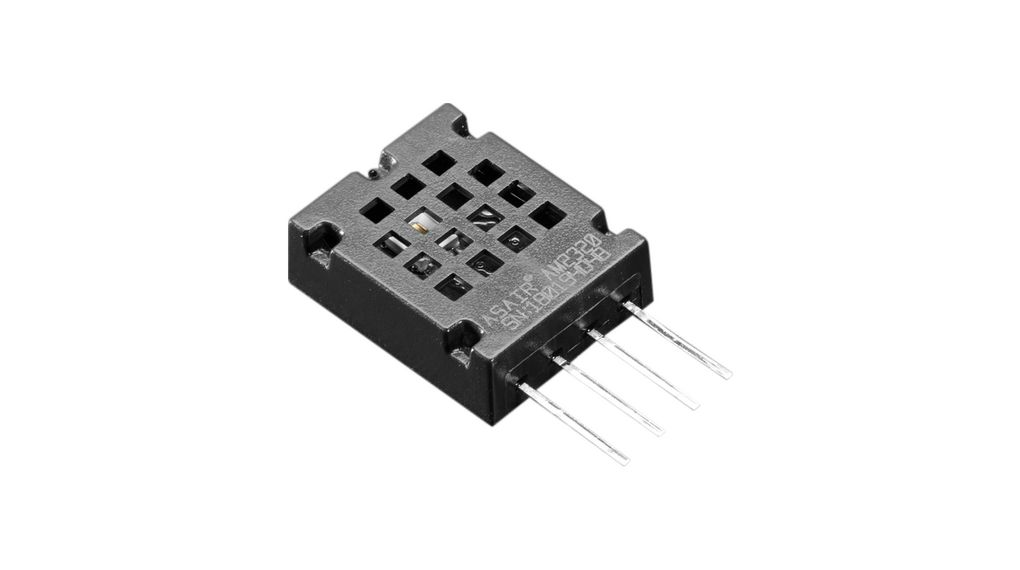
\includegraphics[width=0.25\textwidth]{images/Adafruit-AM2320.jpg}
    \caption{Teploměr a vlhkoměr}
\end{figure}

\subsection{Měření tlaku}
Měření tlaku je zhruba stejně přímočaré jako měření teploty, což znamená, že se o měření stará senzor\cite{tlakoměr},
který je zapojen přes I2C interface, ze kterého program čte hodnotu tlaku v jednotce Pa.

\begin{figure}[h] 
    \centering
    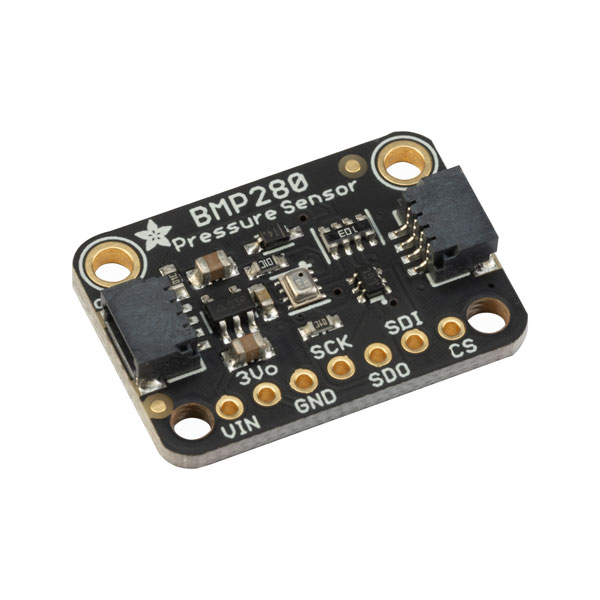
\includegraphics[width=0.25\textwidth]{images/Adafruit-BMP280.jpg}
    \caption{Tlakoměr}
\end{figure}
\subsection{Měření rychlosti větru}
V případě měření rychlosti větru už nestačilo jen koupit senzor, ale bylo potřeba vymyslet jak převést momentum otáčející se osy s lopatkami na reálnou rychlost.
Tento problém je vyřešen následujícím způsobem. Na ose je nasazen disk kruhovitého tvaru, který má v sobě dírky, skrz které optický senzor vysílá paprsek. Pokud se paprsek přeruší,
znamená to, že se mechanismus otočil o jednu dírku. Program tedy počítá kolikrát se paprsek přeruší a spočítá skutečnou rychlost větru pomocí následující rovnice.
\begin{equation}
v = n * d / CasMereni 
\end{equation}
Kde $v$ = rychlost větru, $n$ = počet přerušení, $d$ = vzdálenost uražená větrem na jedno přerušení.

\begin{figure}[h] 
    \centering
    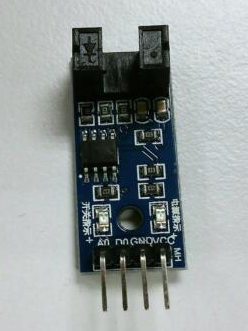
\includegraphics[width=0.25\textwidth]{images/ir_sensor.png}
    \caption{Optická závora}
\end{figure}

\subsection{Měření směru větru}
Měření směru větru je realizováno pomocí magnetického rotačního senzoru, který dokáže měřit odchylku magnetického pole. To bylo využito na měření odchylky větru tak, že na ose, na které je přidělaná střelka, kterou vítr otáčí, je zespod přidělán
malý magnet a senzor tedy měří jeho odchylku.

\begin{figure}[h] 
    \centering
    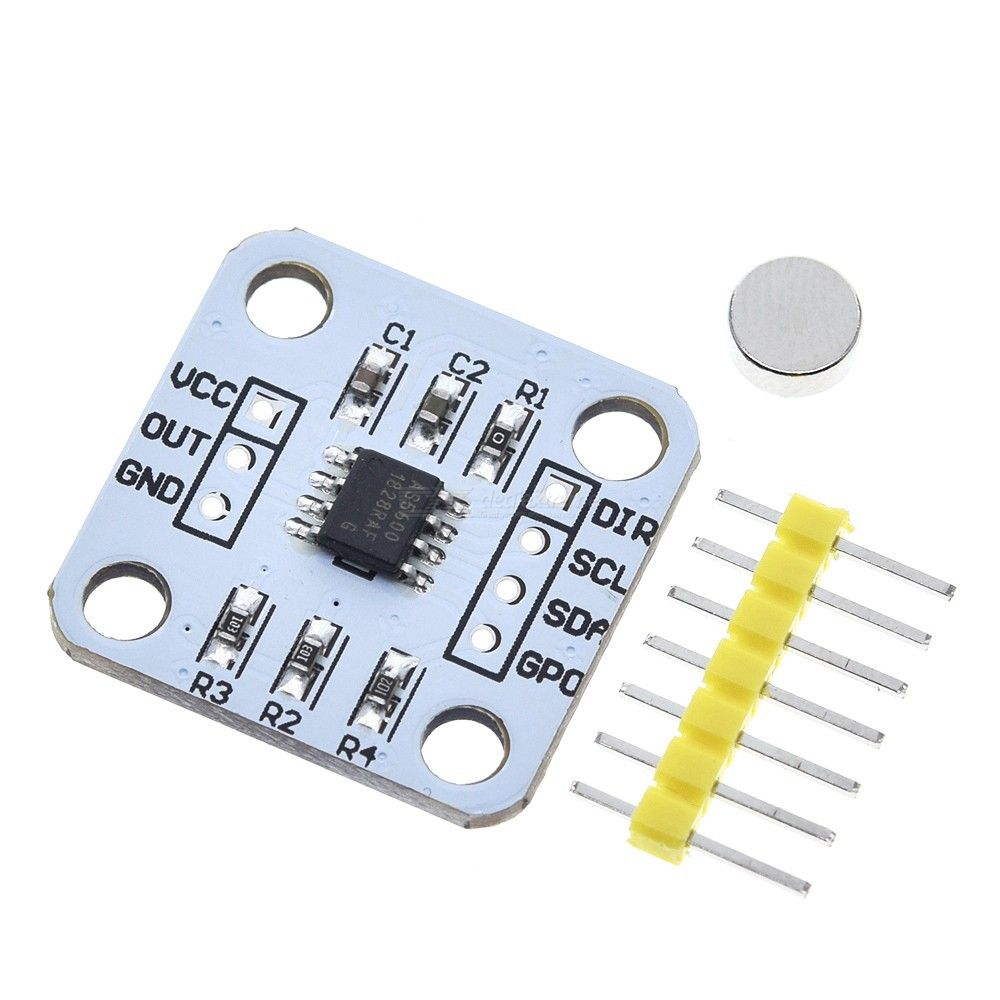
\includegraphics[width=0.25\textwidth]{images/AS5600.jpg}
    \caption{Magnetický rotační senzor}
\end{figure}

\subsection{Měření deště}
Při vytváření součástky na měření deště vzniklo hned několik nápadů jak déšť měřit. Nejprve vznikl nápad, že by skrz trychtýř sbírající vodu prokapávala voda a optický senzor by počítal kapky a tím by měřil déšť.
Tento způsob by však nefungoval, protože optický senzor by nedokázal rozpoznat padající kapku.

Po delším hledání na internetu jsem však našel řešení\cite{mereni_deste}, které by tento problém vyřešilo a nebyl by potřeba žádný optický senzor. Toto řešení spočívá v tom, že voda kape do malé kolébky, která se v jeden moment překlopí a voda kape do druhé strany.
Tímto překlopením kolébka zaktivuje senzor rozpoznání magnetického pole, protože na kolébce je přidělán malý magnet.

\begin{figure}[h] 
    \centering
    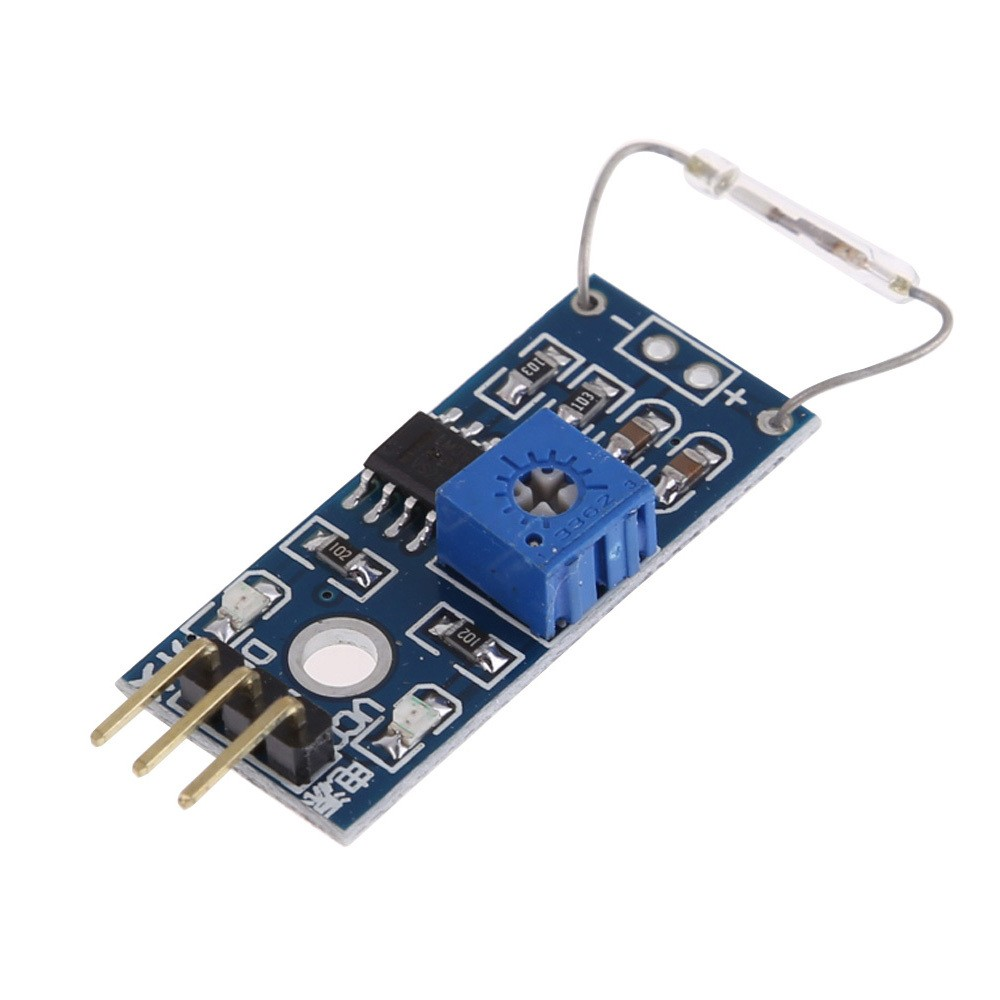
\includegraphics[width=0.25\textwidth]{images/magnet_sensor.jpg}
    \caption{Senzor magnetického pole}
\end{figure}

\subsection{Měření GPS}
Z důvodu, že stanice potřebuje mít informace o své poloze, je ve stanici GPS modul, který získává aktuální GPS souřadnice. Tento senzor má být zapojen na RX/TX piny, ale z důvodu, že na naší arduino desce už
nezbývali volné RX/TX piny, GPS modul musel být zapojen na jiné dva piny a data se z pinů čtou softwarově pomocí knihovny SoftwareSerial. S tímto řešením také ale nastaly první problémy, protože program začal náhodně padat a dlouhou jsem nemohl přijít na příčinu.
Po delším zkoumání jsem přišel na to, že knihovna SoftwareSerial zapisuje data do paměti bez ohledu na to, zda je paměť volná, a tudíž začala přepisovat data programu, což způsobilo padání programu.
Tento problém je dosud nevyřešen, protože už nebyl čas na vytvoření vlastní knihovny, která by tento problém řešila. Další možným řešením by bylo použít jinou desku, která by měla více RX/TX pinů, avšak toto řešení už také nebylo možné.

\subsection{Prostor pro zlepšení}
Největším nedostatek je momentálně neúplná funkce GPS modulu, což by do budoucna chtělo nějakým způsobem vyřešit.
Další možnost pro vylepšení by mohlo být přidání kompasu, protože v tento moment je potřeba natočit stanici správným směrem, aby měřila směr větru přesně. 


